\begin{frame}[fragile]{Tutorial: Two-site states}

\begin{columns}

\begin{column}{4.5cm}

\begin{onlyenv}<1->
%\vspace*{-0.2cm}
\begin{lstlisting}[language=JuliaLocal, style=julia, mathescape, basicstyle=\scriptsize\ttfamily]
i1 = Index(2, "S=1/2,i1")
i2 = Index(2, "S=1/2,i2")

i1 != i2

ZpZm = ITensor(i1, i2)
ZpZm[i1=>1, i2=>2] = 1
\end{lstlisting}
\end{onlyenv}

\begin{onlyenv}<3->
\begin{lstlisting}[language=JuliaLocal, style=julia, basicstyle=\scriptsize\ttfamily]
Zp1=state("Zp",i1)
Zp2=state("Zp",i2)
Zm1=state("Zm",i1)
Zm2=state("Zm",i2)


ZpZm = Zp1 * Zm2
\end{lstlisting}
\end{onlyenv}

\end{column}

\begin{column}{5cm}

\begin{onlyenv}<1-1>
(dim=2|id=505|``S=1/2'') \\
(dim=2|id=576|``S=1/2'') \\
~\\
~\\
~\\
|Z+$\rangle_1$|Z-$\rangle_2$ = |Z+Z-$\rangle$ \\
\end{onlyenv}

\begin{onlyenv}<4->
~\\
~\\
\end{onlyenv}

\begin{onlyenv}<3->
~\\
\end{onlyenv}

\begin{onlyenv}<2->
\vspace*{-0.2cm}
\begin{center}
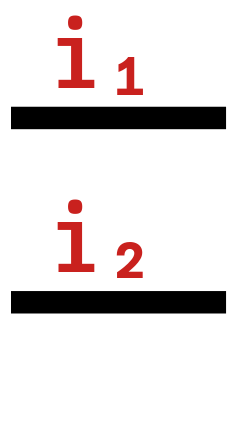
\includegraphics[width=0.225\textwidth]{
  slides/assets/i1i2.png
} \ \ \ \ \ \ \ \ \
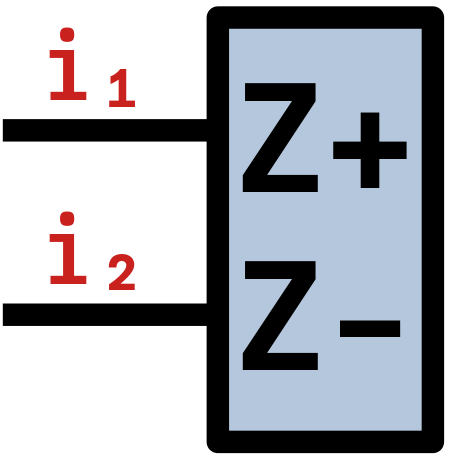
\includegraphics[width=0.4\textwidth]{
  slides/assets/ZpZm12.png
}
\end{center}
\vspace*{0.0cm}
\end{onlyenv}

\begin{onlyenv}<3-3>
~\\
~\\
|Z+$\rangle_1$ \\
|Z+$\rangle_2$ \\
~\\
|Z-$\rangle_1$ \\
|Z-$\rangle_2$ \\
~\\
|Z+Z-$\rangle$ = |Z+$\rangle_1$|Z-$\rangle_2$ \\
~\\
\end{onlyenv}

\begin{onlyenv}<4->
\vspace*{0.0cm}
~\\
\begin{center}
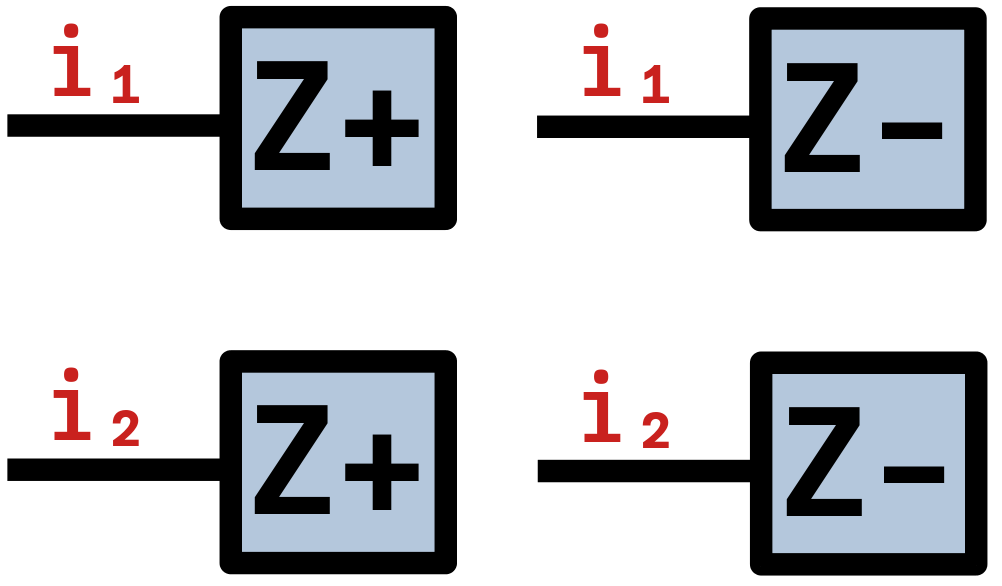
\includegraphics[width=0.5\textwidth]{
  slides/assets/Zp1Zm1Zp2Zm2.png
} \\
~\\
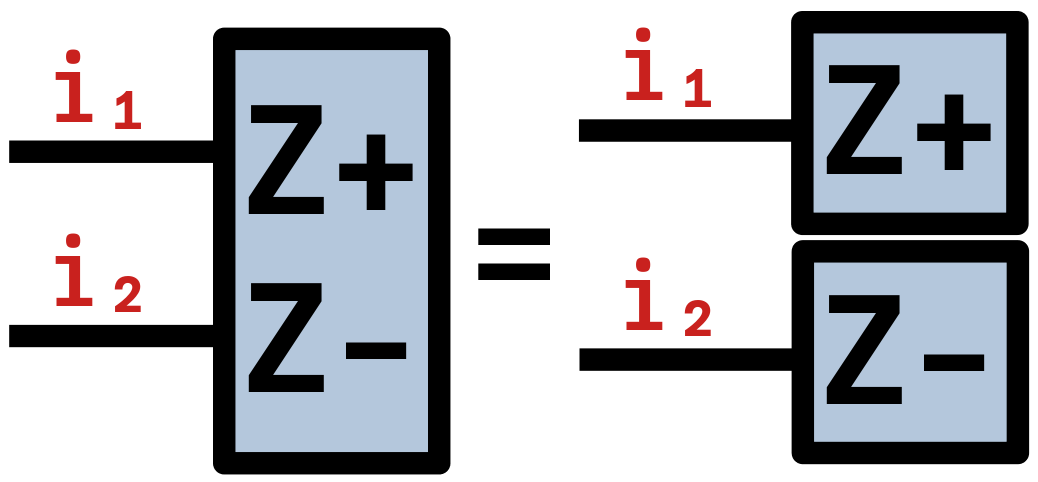
\includegraphics[width=0.5\textwidth]{
  slides/assets/ZpZm12_eq_Zp1Zm2.png
}
\end{center}
\vspace*{0.0cm}
\end{onlyenv}

\end{column}

\end{columns}

\end{frame}
